\documentclass[runningheads,a4paper]{llncs}
\def\spanishoptions{mexico}
\usepackage[spanish]{babel}

\usepackage{amssymb}
\setcounter{tocdepth}{3}
\usepackage{graphicx}
\usepackage[utf8]{inputenc}
\usepackage{url}
\usepackage{listings}
\usepackage[acronyms]{glossaries}
\setacronymstyle{long-short}

\makenoidxglossaries

%Terminos de glosario
\newacronym{NSA}{NSA}{National Security Agency}
\newacronym{CIU}{CIU}{The Competitive Intelligence Unit}
\newacronym{OEA}{OEA}{Organización de los Estados Americanos}
\newacronym{PF}{PF}{Policía Federal}
\newacronym{CMS}{CMS}{Content Management System}
\newacronym{LMS}{LMS}{Learning Management System}
\newacronym{LCMS}{LCMS}{Learning Content Management System}
\newacronym{IMC}{IMC}{Índice Mundial de Ciberseguridad}
\newacronym{TIC}{TIC}{Tecnologías de Información y Comunicaciones}
\newacronym{UIT}{UIT}{Unión Internacional de Telecomunicaciones}
\newacronym{CERT}{CERT}{Computer Emergency Response Team}
\newacronym{CIRT}{CIRT}{Computer Incident Response Team}

\newcommand{\keywords}[1]{\par\addvspace\baselineskip
\noindent\keywordname\enspace\ignorespaces#1}

\begin{document}

\mainmatter  
\title{Introducción de la tesis}
\titlerunning{Introducción de la tesis}
\author{Ing. Felipe de Jesús Miramontes Romero}
\institute{Centro de Investigación en Matemáticas A.C.,\\Maestría en Ingeniería de Software,\\
Avenida Universidad 222, La Loma, 98068, Zacatecas, México.\\felipemiramontesr@gmail.com\\
\url{http://www.ingsoft.mx}}
\maketitle


\begin{abstract}
\keywords{Seguridad cibernetica, Delincuencia informática, México, Técnicas, Estrategias, Planes, Herramientas, Mejora de la Seguridad informática}
\end{abstract}


\section{Introducción de la tesis}
De acuerdo con \cite{Interpol_1} el cibercrimen o delincuencia informática es el área de mas rápido crecimiento dentro de la gama de crímenes punibles de carácter internacional, es perseguida por varias agencias del globo, entre ellas la Interpol y la \gls{NSA} de los Estados Unidos. Los criminales cibernéticos o criminales informáticos aprovechan las potentes capacidades de la tecnología emergente en combinación con técnicas fraudulentas; cometen un diverso rango de actividades criminales, que rompen fronteras e impactan en los aspectos sociales, económicos y políticos del mundo. Se afirma que no existe una definición universal de cibercrimen. Legalmente la ley hace dos distinciones entre los crímenes relacionados a Internet: el primero de ellos es conocido como cibercrimen avanzado ese incluye los crímenes de alta tecnología; por otra parte la llamada ciberdelincuencia habilitada o ``Cyber-Enabled-Crime'' que se enfoca en crímenes de carácter general en los cuales el cibercrimen solo es una herramienta mas para lograr su objetivo: la trata de personas, los crímenes financieros, el narcotráfico y el terrorismo. La Interpol menciona que nuevas tendencias en delincuencia informática están surgiendo todo el tiempo. De acuerdo con \cite{Forbes_1} los costos estimados para la economía mundial por estos crímenes están entre los 375 y los 575 mil millones de dolares al año.\\

De acuerdo con la Interpol \cite{Interpol_1} hace algunos años los delitos cibernéticos eran cometidos principalmente por individuos o grupos pequeños. Hoy en día existen redes complejas de criminales que pretenden reunir a personas de todo el mundo en tiempo real para cometer crímenes en una escala sin precedentes.\\

En México, Enrique Galindo Ceballos, comisionado general de la Policía Federal de México en 2015 ha declarado en conferencia de prensa \cite{Forbes_1} que es fundamental controlar la integridad y confidencialidad de la información pues la mayoría de los sectores de economía y gobierno del país basan su completa operación en la afamada red mundial. Durante la presentación de los resultados de la estrategia nacional de ciberseguridad, el funcionario declaró que con el desarrollo de las tecnologías de información, los gobiernos han establecido al ciberespacio como un nuevo entorno operativo, por lo que actualmente controlar la integridad, disponibilidad y confidencialidad de la información se vuelve un tema fundamental en lo económico y político de las naciones. Ademas se dijo que del 1 de diciembre del 2012 al 1 de febrero del 2015 se emitieron más de 1,000 alertas de seguridad que permitieron prevenir y mitigar incidentes cibernéticos gracias a la colaboración internacional, así mismo se lograron atender de diciembre de 2012 a enero 2015, aproximadamente 59,236 incidentes cibernéticos. Así mismo se hizo referencia a la siguiente información de de alto impacto: 

\begin{enumerate}
	\item El 53\% de los incidentes cibernéticos identificados fueron en contra de los tres órdenes de gobierno, 26\% al ámbito académico y 21\% al privado.\\
	\item Las principales afectaciones son, 68\% suplantación y robo de identidad, 17\% fraude cibernético, 15\% ataques a sitios web.\\
	\item A pesar de la complejidad para la persecución de estos delitos, se cumplimentaron 47 órdenes de cateo y fueron detenidos 36 probables responsables.\\
	\item El patrullaje virtual de la \gls{PF} identificó y desactivó 5,549 sitios web apócrifos usurpadores de instancias financieras y de gobierno.
\end{enumerate}

De acuerdo a Kapellmann y Reyes \cite{RCM_1}, la consultora \gls{CIU} afirma que, ``por medio de la Reforma en Materia de Telecomunicaciones \cite{RMT_1} y la Estrategia Digital Nacional \cite{EDN_1} se ha dado prioridad a la digitalización de la población y los servicios públicos, pero el tema de la ciberseguridad no ha recibido el mismo ímpetu''. Ademas se dice que en 2014 México contó con una calificación global en seguridad informática de 32.4 sobre 100, lo cual implica que se encuentra 12.3 puntos por debajo del promedio global. A nivel latinoamérica México se ubica por encima de países como Paraguay y Venezuela, pero muy por debajo de otros como Brasil, Uruguay, Argentina, Costa Rica, Chile y Colombia. Según el reporte ``Tendencias de Seguridad en América Latina y el Caribe'' \cite{TSCALC_1}, de la \gls{OEA}, en México los costos anuales generados por ciberdelitos en 2014 ascendieron a 3 mil millones de dólares, afectando a los sectores público, privado y civil. ABI Research \cite{GCSI_1} afirma que el \gls{IMC} es una medida del nivel de desarrollo de la ciberseguridad de cada estado nación y ha sido creado con el fin de fomentar una cultura mundial en pro de la seguridad informática y de la integración de las \gls{TIC} como elemento catalizador. Brahima Sanou \cite{GCSI_1} menciona que el \gls{IMC} ha sido calculado en colaboración con ABI Research, institución especializada en análisis estadísticos y evaluación comparativa de las industrias, quienes han desarrollado cuestionarios especializados para la extracción de información; y sus resultados fueron presentados a todos los Estados Miembros de la \gls{UIT}. Dentro de su metodología se realizaron encuestas a nivel de país, complementadas con una investigación cualitativa a fondo; se recopilo información sobre leyes, reglamentos; \gls{CERT} y \gls{CIRT}, políticas, estrategias nacionales, normas, certificaciones, formación profesional, sensibilización, y asociaciones de colaboración. Otorgando una calificación a cada país miembro. Para la calificación se tomaron en cuenta 5 áreas especificas: medidas jurídicas, medidas técnicas, medidas de organización, creación de capacidades y cooperación. \\

A continuación es presentado un resumen de resultados del \gls{IMC} 2015 (Figuras 1 y 2), en el cual son presentados los 5 países con mejor calificación, los 5 países con peor calificación y un rango de 5 países en el cual aparece México. Los datos mostrados hacen referencia a la calificación denominada Índice la cual se compone de la ponderación de las áreas mencionadas anteriormente, además se muestra la clasificación de cada país la cual indica su posición en la tabla general de calificaciones. Los detalles del estudio \gls{IMC} se encuentran en \cite{GCSI_1}.\\

\begin{figure}
\centering
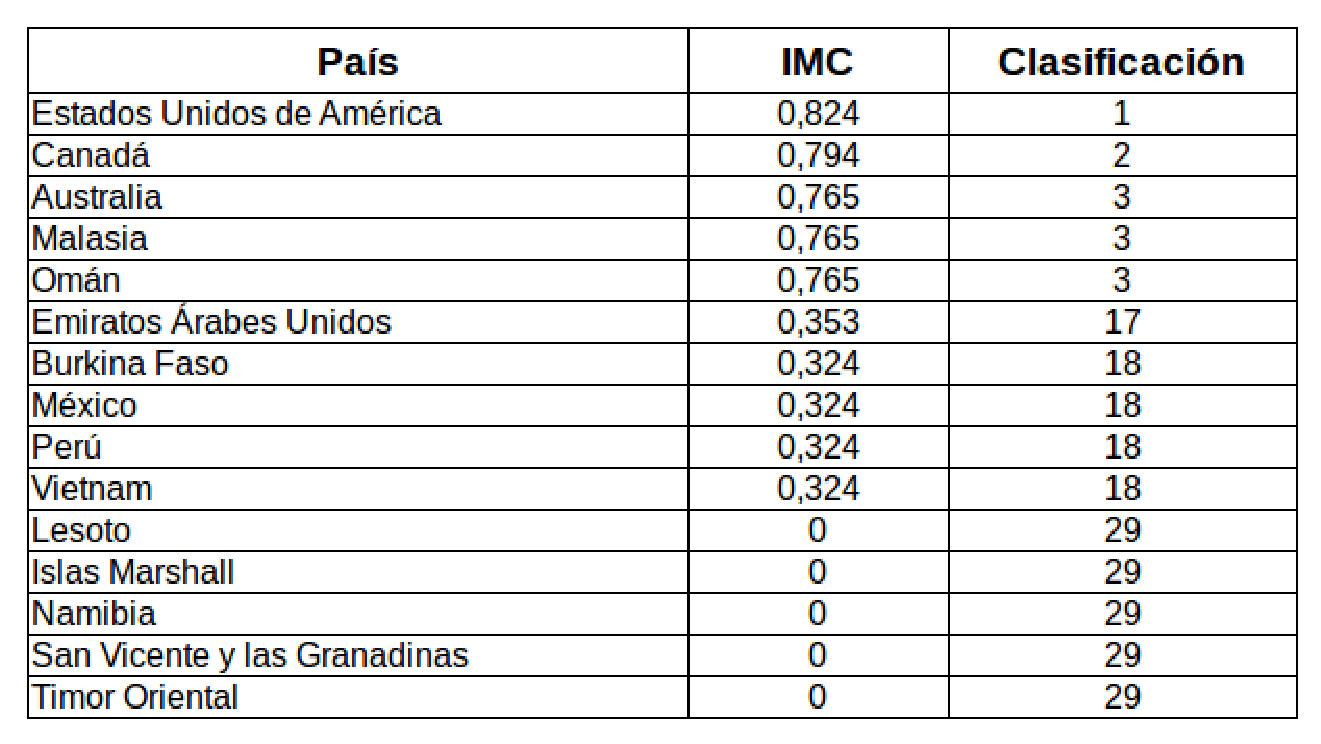
\includegraphics[height=6.5cm, width=12.0cm]{imc}
\caption{Indice Mundial de Ciberseguridad}
\label{fig:example}
\end{figure}


\begin{figure}
\centering
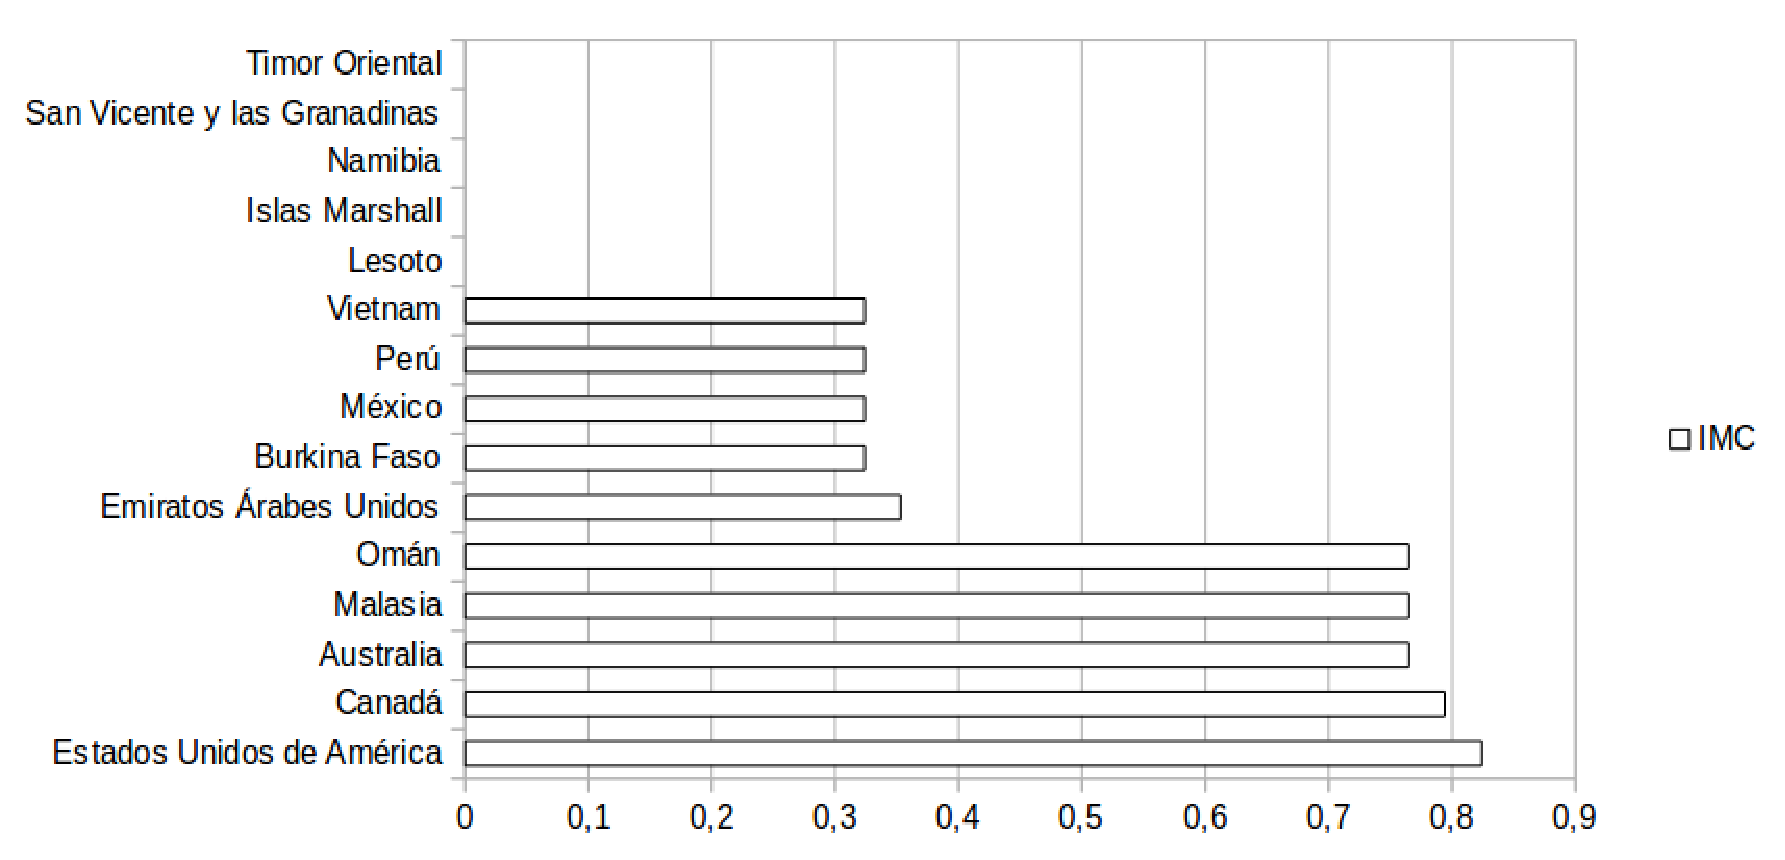
\includegraphics[height=6.5cm, width=12.0cm]{imc_graph}
\caption{Comparativa del Indice Mundial de Ciberseguridad (IMC).}
\label{fig:example}
\end{figure}

En ``Retos de Ciberseguridad para México'' \cite{RCM_1} , se dice que es de suma importancia comenzar con la pronta elaboración e implementación de estrategias y planes nacionales que agilicen la transición hacia un ciberespacio seguro, donde sea posible aprovechar los beneficios que generan las tecnologías de información y comunicaciones. En este documento es presentado un modelo de trabajo que pretende satisfacer las necesidades actuales de los principales afectados por medio de la supresión de la mayor cantidad de vulnerabilidades durante el ciclo de vida de desarrollo de sistemas web basados en plataformas \gls{CMS}, \gls{LMS}, \gls{LCMS} y e-Commerce. Para lograr un correcto entendimiento de la panorámica general se han realizado en este trabajo actividades y experimentos con el fin de comprender la simbiosis cibernética existente entre los mecanismos que actualmente son utilizados en pro de la mejora de la seguridad de la información en los sistemas web localizados geográficamente en México.\\

El presente trabajo se encuentra estructurado de una manera simple y en el se encuentran contenidas las siguientes secciones:

\begin{itemize}
	\item Antecedentes; en esta sección es posible encontrar la información necesaria para comprender el panorama tecnológico actual de México; es decir, los resultados obtenidos de los experimentos y estudios realizados para responder la interrogante: ¿Qué se ha hecho a favor de la construcción de sistemas web seguros en México? Ademas de ello, es posible encontrar el planteamiento del problema que se ha identificado, los objetivos generales, específicos y la justificación del desarrollo de la propuesta.\\
	
	\item Estado de arte; según Molina \cite{La_salle_1} en esta sección se aborda la información que da respuesta a la interrogación: ¿Cómo fue realizado el estudio del conocimiento acumulado (escrito en textos)? Dicha información pertenece a la rama de la tecnología denominada seguridad informática, en la especialidad de desarrollo de sistemas web seguros.\\
	
	\item Propuesta; en esta sección se aborda a detalle la información relacionada al modelo de trabajo propuesto.\\
	
	\item Caso de estudio; en esta sección es posible localizar la información concerniente al desarrollo de un sistema web seguro utilizando el modelo de trabajo propuesto, esto con el fin de poder evaluar el impacto del mismo en un entorno real. \\
	
	\item Resultados; en esta sección es posible encontrar los datos obtenidos de la evaluación de la propuesta, así como la información relacionada con la medición del impacto en la seguridad de la información en México.\\
	
	\item Conclusiones; en esta sección es posible encontrar los aprendizajes generales de la interacción y el desarrollo de los mecanismos incluidos en la propuesta, así como el trabajo hacia el futuro, así como la áreas de oportunidad de la aplicación para el presente trabajo.
\end{itemize} 


\printnoidxglossaries     
         
\bibliographystyle{ieeetr}
\bibliography{bibliography}


\end{document}
